\documentclass[conf]{new-aiaa}
\usepackage[utf8]{inputenc}
\usepackage{graphicx}
\usepackage{amsmath}
\usepackage{amssymb}
\usepackage{longtable,tabularx}
\usepackage{booktabs}
\usepackage{tikz}
\usepackage{multirow}
\usepackage{xcolor}
\usetikzlibrary{shapes.geometric, arrows.meta, positioning}
\setlength\LTleft{0pt}

\title{Surface-Object Detection and Tracking from Commercial X-Band Marine Radar Using Adaptive ST-DBSCAN}

\author{Samuel Cancilla\footnote{Undergraduate Research Assistant, Department of Mechanical Engineering, AIAA Student Member.}, J.C. Vaught\footnote{Graduate Research Assistant, Department of Mechanical Engineering.}, Douglas Cahl\footnote{Research Associate, Department of Mechanical Engineering.}, and Yi Wang\footnote{Associate Professor, Department of Mechanical Engineering, AIAA Associate Fellow.}}
\affil{University of South Carolina, Columbia, SC 29208}

\begin{document}

\maketitle

\begin{abstract}
Maritime missions such as over-water navigation, ship-based operations, and airborne/space-enabled maritime surveillance require reliable surface-object detection and tracking in the presence of strong, nonstationary sea clutter and intermittent object returns. We present an end-to-end, real-time pipeline for vessel detection and multi-sweep tracking using commercial X-band radar providing only intensity measurements (range, azimuth, and intensity) without Doppler phase history. Raw polar returns from a Furuno NXT solid-state unit are transformed into Cartesian point clouds and clustered using ST-DBSCAN to link detections across sweeps. Neighborhood radii adapt automatically via k-nearest-neighbor distance statistics to handle varying clutter and point densities. A lightweight gap-recovery mechanism reconnects clusters across brief temporal dropouts. We evaluate the approach on (i) a synthetic dataset with ground-truth trajectories and (ii) coastal radar data from a shore-mounted installation, characterizing detection-to-track association behavior relative to baseline DBSCAN and standard ST-DBSCAN under nonstationary clutter and intermittent returns. A Rust implementation runs at 2 sweeps/s on an NVIDIA Jetson Orin, exceeding real-time requirements for a 48 RPM radar.
\end{abstract}

%% ============================================================================
%% NOMENCLATURE
%% ============================================================================
\section{Nomenclature}

{\renewcommand\arraystretch{1.0}
\noindent\begin{longtable*}{@{}l @{\quad=\quad} l@{}}
$\varepsilon_s$ & spatial neighborhood radius for clustering (pixels) \\
$\varepsilon_t$ & temporal neighborhood radius (number of frames) \\
$N_{\min}$ & minimum number of neighbors required for a core point \\
$k$ & number of nearest neighbors for adaptive radius estimation \\
$d_k(\mathbf{p})$ & distance to $k$-th nearest neighbor of point $\mathbf{p}$ \\
$d(\mathbf{p}, \mathbf{q})$ & Euclidean distance between points $\mathbf{p}$ and $\mathbf{q}$ \\
$\mathbf{p}_i$ & radar point with coordinates $(x_i, y_i)$ and frame index $t_i$ \\
$d_{\max}$ & maximum distance threshold for track-to-cluster association \\
$d_{\text{gap}}$ & maximum centroid distance for gap recovery (pixels) \\
$\tau_{\max}$ & maximum track age before deletion (frames) \\
$\tau_{\text{gap}}$ & maximum gap duration for cluster reconnection (frames)
\end{longtable*}}

%% ============================================================================
%% INTRODUCTION
%% ============================================================================
\section{Introduction}

When a small vessel enters a wave trough off the South Carolina coast, its radar return vanishes for two or three antenna sweeps. A conventional tracking system, seeing no detections, increments the track's age counter; after several more dropouts caused by wave shadowing and radar cross-section fluctuations, the system deletes the track entirely. Moments later, the vessel reappears---but now as a new track with a fresh identifier, its previous history lost. This scenario, repeated across dozens of vessels during a typical harbor approach, degrades situational awareness precisely when it matters most.

Maritime domain awareness is essential for navigation safety, port security, and search-and-rescue operations. Commercial X-band marine radars operating at 9.3--9.5~GHz provide reliable all-weather sensing of surface vessels and other objects of interest. However, extracting consistent object tracks from raw radar data remains challenging due to sea clutter, multipath reflections, and the intermittent target visibility illustrated above.

Traditional radar processing pipelines employ Constant False Alarm Rate (CFAR) detection followed by kinematic filtering using Kalman or alpha-beta trackers~\cite{rohling1983radar, bar2011tracking}. While effective for isolated targets in open water, these methods struggle with dense vessel traffic and the nonstationary clutter conditions common in coastal waters. CFAR detectors require careful threshold tuning for each environment, and single-frame detection discards valuable temporal information that could link fragmented returns across sweeps.

The increasing availability of solid-state marine radars with high range resolution (sub-meter) and fast scan rates (24--48 RPM) motivates point-cloud-based processing approaches that exploit both spatial and temporal coherence. Unlike traditional plot extraction, which reduces each target to a single position estimate per scan, point cloud methods preserve the spatial extent of radar returns, enabling better discrimination of closely spaced targets and more robust association across frames.

This paper presents an end-to-end detection and tracking system based on an adaptive variant of Spatio-Temporal DBSCAN (ST-DBSCAN) clustering. The main contributions include an adaptive ST-DBSCAN formulation where neighborhood radii are estimated automatically from k-nearest-neighbor distance statistics, eliminating manual parameter tuning for different clutter environments; a gap-recovery mechanism that reconnects clusters across brief temporal dropouts caused by intermittent radar returns; an efficient implementation combining spatial hashing for $O(1)$ average-case neighbor queries with union-find for cluster merging; and experimental evaluation on synthetic scenarios with ground-truth trajectories and real coastal radar data, characterizing tracking behavior under varying conditions.


%% ============================================================================
%% RELATED WORK
%% ============================================================================
\section{Related Work}

\subsection{Radar Target Detection}

Traditional marine radar processing uses CFAR detection to identify targets against sea clutter and thermal noise~\cite{rohling1983radar}. Cell-averaging CFAR (CA-CFAR) estimates local noise power from neighboring range cells and sets a detection threshold accordingly. While effective in homogeneous clutter, CA-CFAR suffers from target masking in dense traffic and requires environment-specific tuning.

Recent advances in solid-state radar technology have motivated point-cloud-based processing approaches. Vivone et al.~\cite{vivone2016sar} demonstrated multi-target tracking from synthetic aperture radar using density-based clustering. In the automotive domain, radar point cloud processing has benefited from deep learning approaches, though these require extensive labeled training data not typically available for maritime applications.

\subsection{Density-Based Clustering}

DBSCAN (Density-Based Spatial Clustering of Applications with Noise), introduced by Ester et al.~\cite{ester1996density}, identifies clusters as regions of high point density separated by regions of low density. The algorithm classifies each point as either a \textit{core point} (having at least $N_{\min}$ neighbors within distance $\varepsilon$), a \textit{border point} (within $\varepsilon$ of a core point but not itself a core point), or \textit{noise}.

ST-DBSCAN~\cite{birant2007st} extends DBSCAN to spatio-temporal data by introducing separate thresholds for spatial ($\varepsilon_s$) and temporal ($\varepsilon_t$) dimensions. Points must satisfy both spatial and temporal proximity to be considered neighbors, preventing merging of spatially close but temporally distant points---essential for tracking moving objects.

A key limitation of standard DBSCAN is sensitivity to the choice of $\varepsilon$. Several extensions address this: OPTICS~\cite{ankerst1999optics} produces a reachability ordering that can be cut at various density thresholds, while HDBSCAN~\cite{campello2013hdbscan} constructs a cluster hierarchy and extracts stable clusters automatically. Our k-nearest-neighbor approach to adaptive $\varepsilon$ estimation is related to the common ``elbow method'' for DBSCAN parameter selection, but we apply it in real-time to each frame rather than as an offline preprocessing step.

\subsection{Multi-Object Tracking}

Multi-object tracking (MOT) maintains object identities across time by solving the data association problem---matching new detections to existing tracks~\cite{bar2011tracking}. The Hungarian algorithm~\cite{kuhn1955hungarian} provides a globally optimal solution in $O(n^3)$ time.

Joint Probabilistic Data Association (JPDA)~\cite{bar2004jpda} handles measurement-to-track association uncertainty by computing weighted updates across all plausible associations. For extended targets producing multiple measurements, Probability Hypothesis Density (PHD) filters~\cite{mahler2003phd} provide principled approaches to multi-object tracking. Recent work on Simple Online and Realtime Tracking (SORT)~\cite{bewley2016sort} demonstrates that combining simple motion models with optimal assignment can achieve competitive performance at real-time rates, motivating our Hungarian-based approach.

%% ============================================================================
%% METHODOLOGY
%% ============================================================================
\section{Methodology}

The processing pipeline consists of four stages: (1)~point cloud extraction from radar imagery, (2)~adaptive parameter estimation, (3)~spatio-temporal clustering with gap recovery, and (4)~multi-object tracking. Figure~\ref{fig:pipeline} illustrates the system architecture.

\begin{figure}[hbt!]
\centering
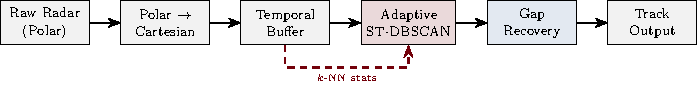
\includegraphics[width=\linewidth]{figures/fig_pipeline.pdf}
\caption{Processing pipeline from polar radar returns to tracked objects. Raw polar data is transformed into Cartesian point clouds, clustered using adaptive ST-DBSCAN with gap recovery, and tracked via Hungarian assignment.}
\label{fig:pipeline}
\end{figure}

\subsection{Point Cloud Generation}

The Furuno DRS-NXT radar outputs Plan Position Indicator (PPI) images as 8-bit grayscale bitmaps representing received signal intensity. Unlike Doppler radars, the unit provides only intensity measurements without phase history. The preprocessing stage converts polar radar data to Cartesian point clouds through four operations. First, raw returns in $(r, \theta)$ coordinates are converted to Cartesian $(x, y)$ using standard trigonometric projection. Second, intensity thresholding discards pixels with intensity $I < I_{\text{thresh}}$ where $I_{\text{thresh}} = 25$ (10\% of maximum for 8-bit data). Third, stride-based subsampling with stride $s=2$ reduces point count by 75\% with negligible impact on clustering quality. Finally, each point is assigned a frame identifier $t_i$ corresponding to the radar sweep number.

A typical sweep produces 12,000--50,000 points after preprocessing.

\begin{figure}[hbt!]
\centering
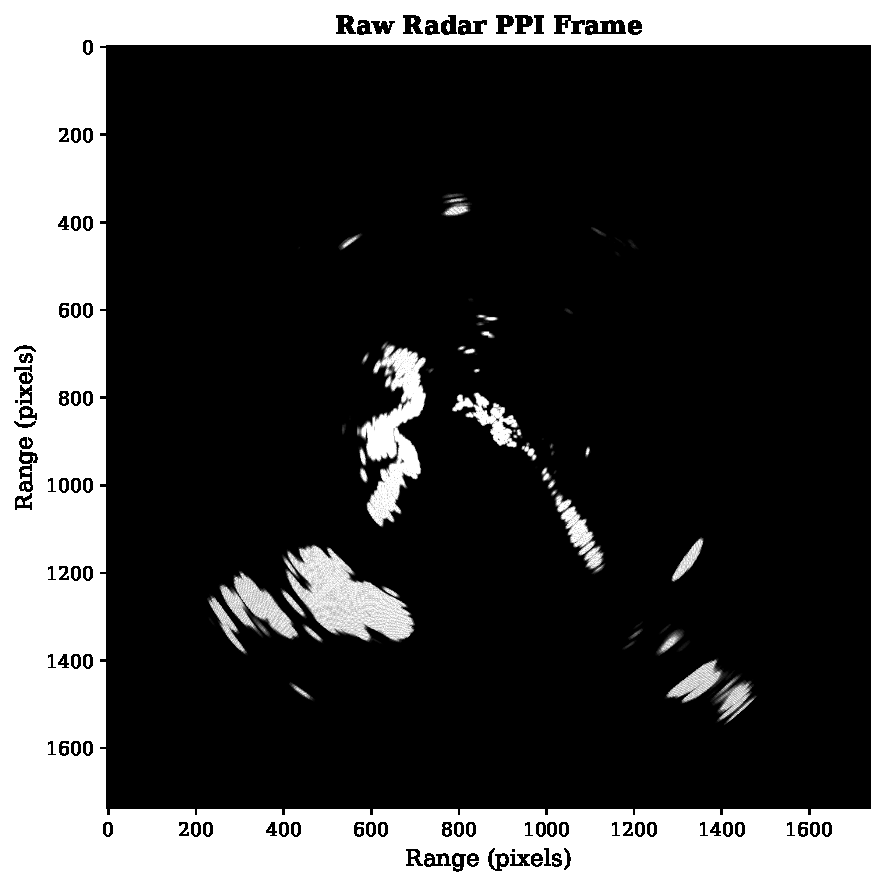
\includegraphics[width=0.85\linewidth]{figures/fig_raw_radar.pdf}
\caption{Raw radar return example from the Furuno DRS-NXT unit. Multiple vessel returns are visible against varying sea clutter intensity, demonstrating the challenging detection environment.}
\label{fig:raw_radar}
\end{figure}

\begin{figure}[hbt!]
\centering
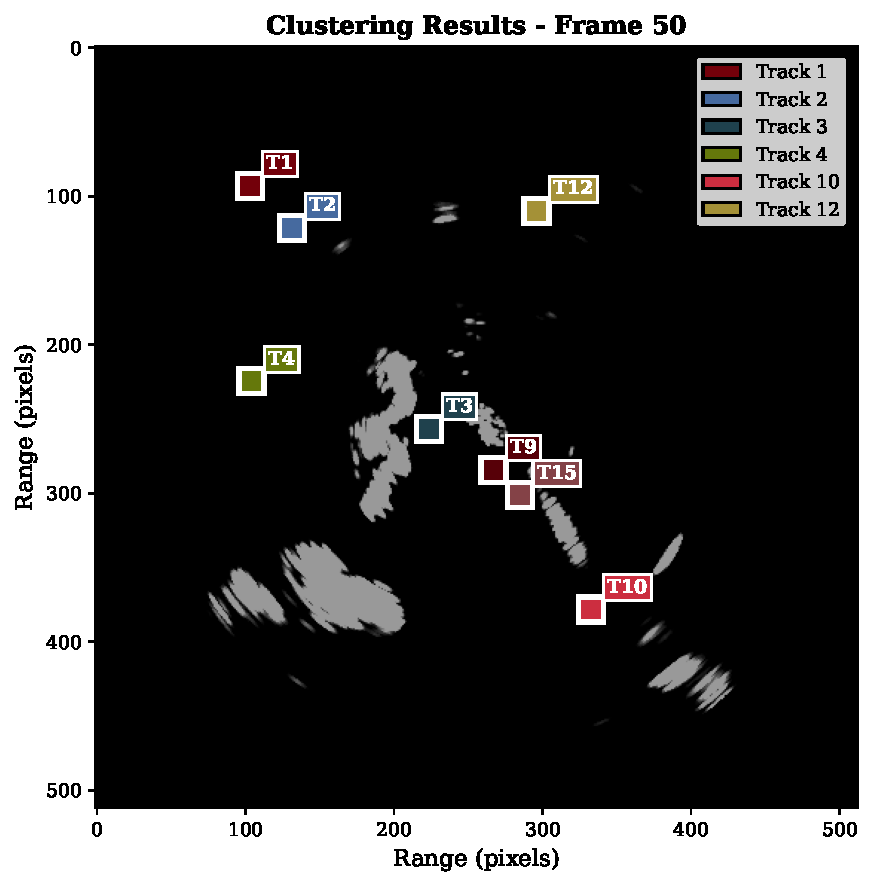
\includegraphics[width=0.85\linewidth]{figures/fig_clustering_result.pdf}
\caption{ST-DBSCAN clustering result on a multi-vessel scene. Each cluster is assigned a unique color; noise points are shown in gray. The algorithm successfully separates individual vessel returns from sea clutter.}
\label{fig:clustering_result}
\end{figure}

\subsection{Adaptive Parameter Estimation}

Standard ST-DBSCAN requires manual selection of $\varepsilon_s$, which is sensitive to local point density. We propose automatic estimation using k-nearest-neighbor (k-NN) distance statistics.

For each point $\mathbf{p}$, let $d_k(\mathbf{p})$ denote the distance to its $k$-th nearest spatial neighbor. The distribution of $d_k$ values across all points characterizes local density. We estimate $\varepsilon_s$ as:
\begin{equation}
\varepsilon_s = \text{percentile}_{90}\left( \{ d_k(\mathbf{p}) : \mathbf{p} \in \mathcal{P} \} \right)
\end{equation}
where $k = N_{\min}$ (typically 5). This choice ensures that approximately 90\% of points have sufficient neighbors to potentially become core points, while rejecting the sparsest 10\% as likely noise.

The k-NN distances are computed efficiently using the same spatial hash structure used for clustering, yielding $O(n)$ average-case complexity for parameter estimation.

\subsection{ST-DBSCAN Clustering}

The neighborhood of a point $\mathbf{p}$ is defined as:
\begin{equation}
\mathcal{N}(\mathbf{p}) = \left\{ \mathbf{q} \in \mathcal{P} : d(\mathbf{p}, \mathbf{q}) \leq \varepsilon_s \;\land\; |t_{\mathbf{p}} - t_{\mathbf{q}}| \leq \varepsilon_t \right\}
\end{equation}

A point is a \textit{core point} if $|\mathcal{N}(\mathbf{p})| \geq N_{\min}$. Clusters form by connecting density-reachable core points. Border points join their nearest core point's cluster; isolated points are labeled as noise.

Setting $\varepsilon_t = 2$ links detections across five consecutive frames, improving cluster coherence when individual frames have sparse returns.

\subsubsection{Spatial Hashing}

We use a spatial hash grid that partitions the 3D space $(x, y, t)$ into cells of size $\varepsilon_s$:
\begin{equation}
\text{cell}(\mathbf{p}) = \left( \left\lfloor \frac{x}{\varepsilon_s} \right\rfloor, \; \left\lfloor \frac{y}{\varepsilon_s} \right\rfloor, \; t \right)
\end{equation}

All spatial neighbors lie within 27 cells (3$\times$3$\times$3 in space-time). For uniformly distributed points, this yields $O(1)$ average-case neighbor queries.

\subsubsection{Union-Find for Cluster Merging}

Connected core points merge using a union-find data structure with path compression and union by rank, yielding $O(\alpha(n))$ amortized time per operation where $\alpha$ is the inverse Ackermann function.

\subsection{Gap Recovery Mechanism}

Intermittent radar returns cause temporal gaps where a vessel produces no detectable points for one or more sweeps. Standard ST-DBSCAN with $\varepsilon_t = 2$ handles gaps up to 2 frames, but longer dropouts fragment clusters. We propose a lightweight gap-recovery post-processing step in which we first identify cluster pairs $(C_i, C_j)$ where $C_i$ ends at frame $t_1$ and $C_j$ begins at frame $t_2$ with temporal separation $t_2 - t_1 \leq \tau_{\text{gap}}$ (gap threshold, typically 5 frames) and spatial centroids satisfying $\| \bar{\mathbf{x}}_i - \bar{\mathbf{x}}_j \| < d_{\text{gap}}$. Qualifying cluster pairs are then merged by relabeling $C_j$ points with $C_i$'s cluster ID. This reconnects clusters across dropouts of up to $\tau_{\text{gap}}$ frames without modifying the core ST-DBSCAN algorithm.

\begin{figure}[hbt!]
\centering
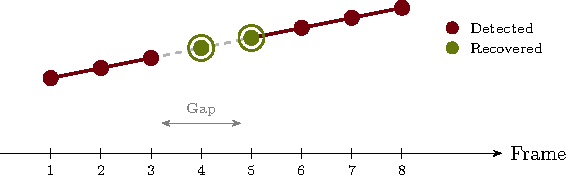
\includegraphics[width=0.9\linewidth]{figures/fig_gap.pdf}
\caption{Gap recovery mechanism. When a vessel temporarily disappears (frames $t_1$ to $t_2$), the algorithm reconnects clusters based on centroid proximity, maintaining track identity across brief dropouts.}
\label{fig:gap}
\end{figure}

\subsection{Multi-Object Tracking}

The tracking module maintains persistent object identities using a predict-associate-update cycle.

\subsubsection{Motion Model}

Each track maintains a velocity estimate using exponential smoothing:
\begin{equation}
\mathbf{v}_{k} = \alpha \cdot (\mathbf{x}_k - \mathbf{x}_{k-1}) + (1 - \alpha) \cdot \mathbf{v}_{k-1}
\end{equation}
where $\alpha = 0.7$. The predicted position is $\hat{\mathbf{x}}_{k+1} = \mathbf{x}_k + \mathbf{v}_k$.

\subsubsection{Hungarian Assignment}

The cost of assigning track $i$ to cluster $j$ is the Euclidean distance $C_{ij} = \| \hat{\mathbf{x}}_i - \mathbf{c}_j \|$. The Hungarian algorithm finds globally optimal one-to-one assignments in $O(m^3)$ time.

\subsubsection{Track Lifecycle}

Track management follows a three-state lifecycle: unmatched clusters spawn new tracks upon first detection; matched tracks update their position and velocity estimates while resetting their age counter; and tracks exceeding $\tau_{\max}$ consecutive unmatched frames are deleted from the active track set.

\begin{figure}[hbt!]
\centering
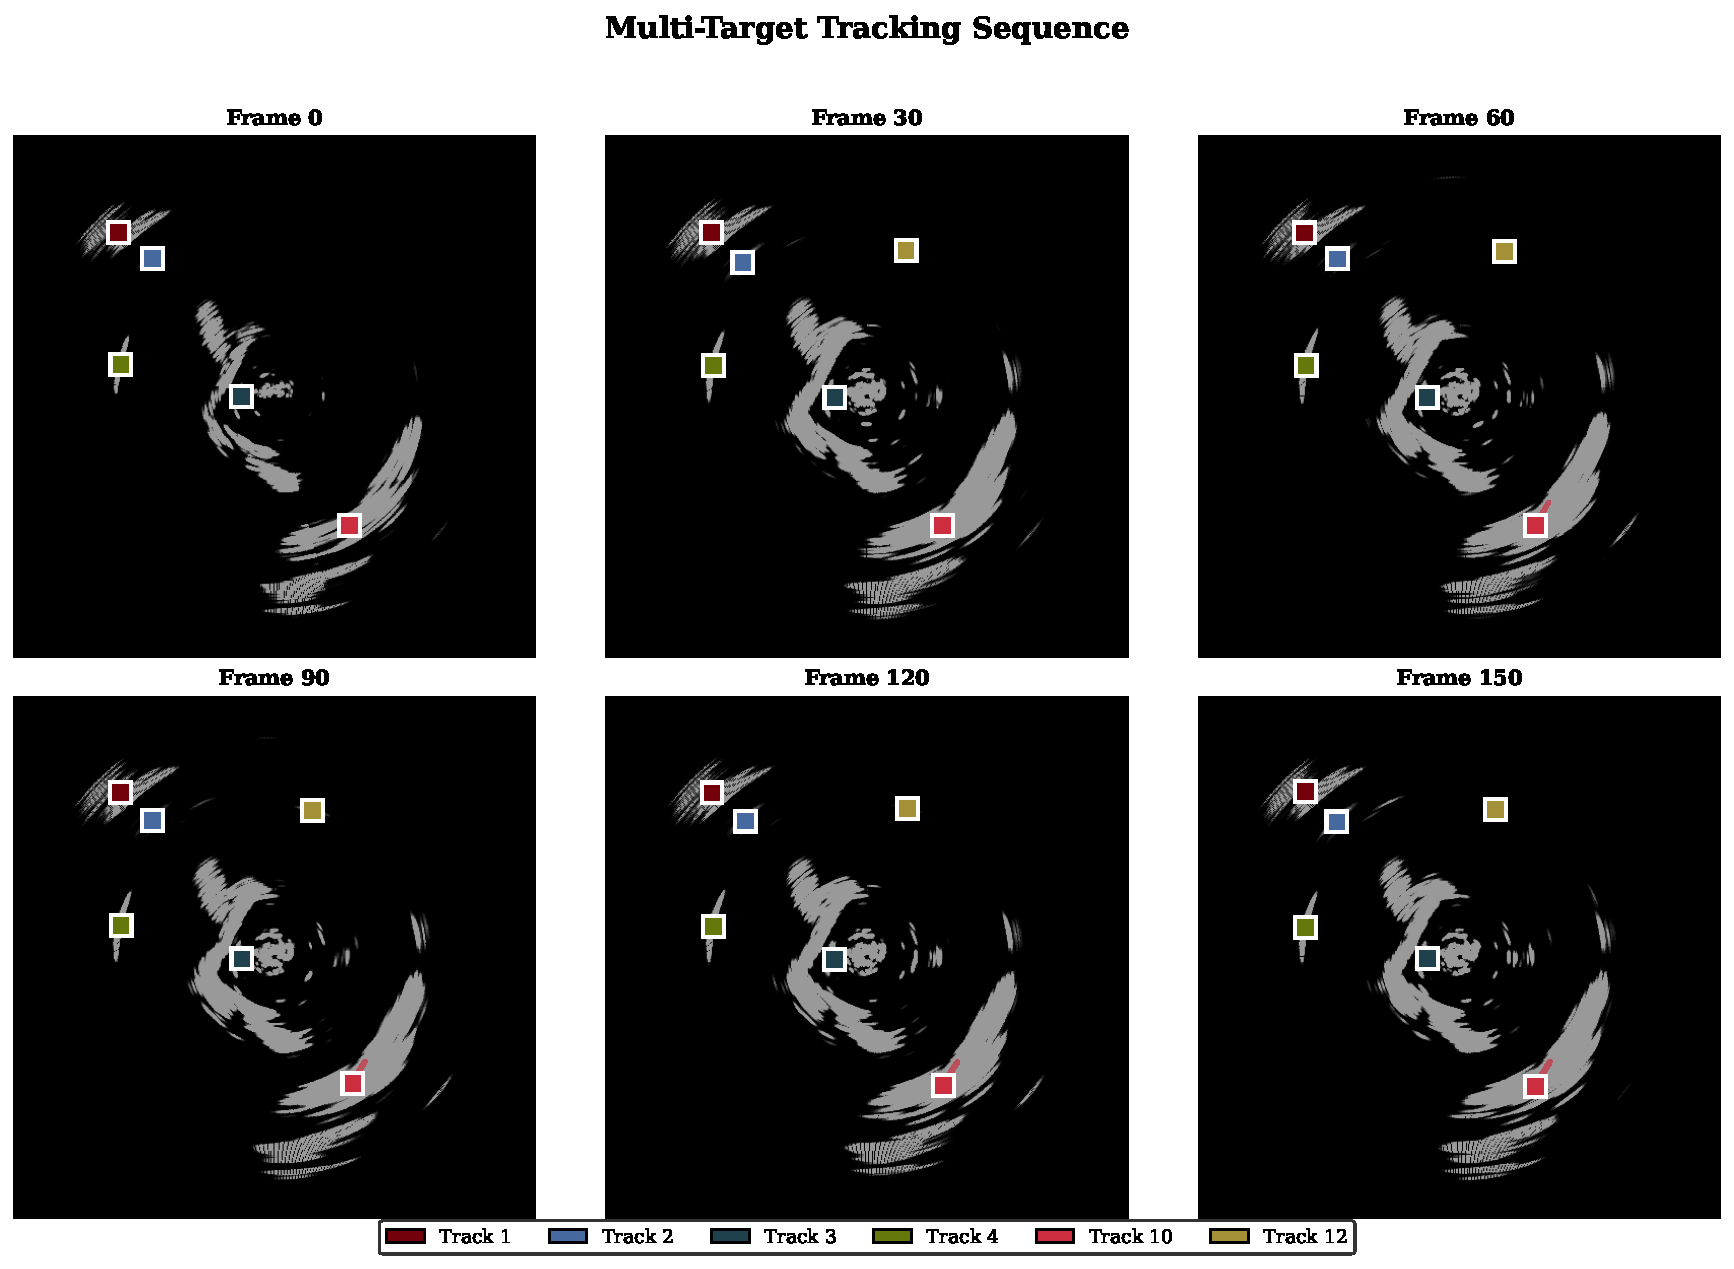
\includegraphics[width=\linewidth]{figures/fig_tracking_sequence.pdf}
\caption{Tracking sequence showing vessel positions across consecutive radar sweeps. Track identifiers remain consistent despite intermittent detections, demonstrating the effectiveness of the gap recovery mechanism.}
\label{fig:tracking_sequence}
\end{figure}

\begin{figure}[hbt!]
\centering
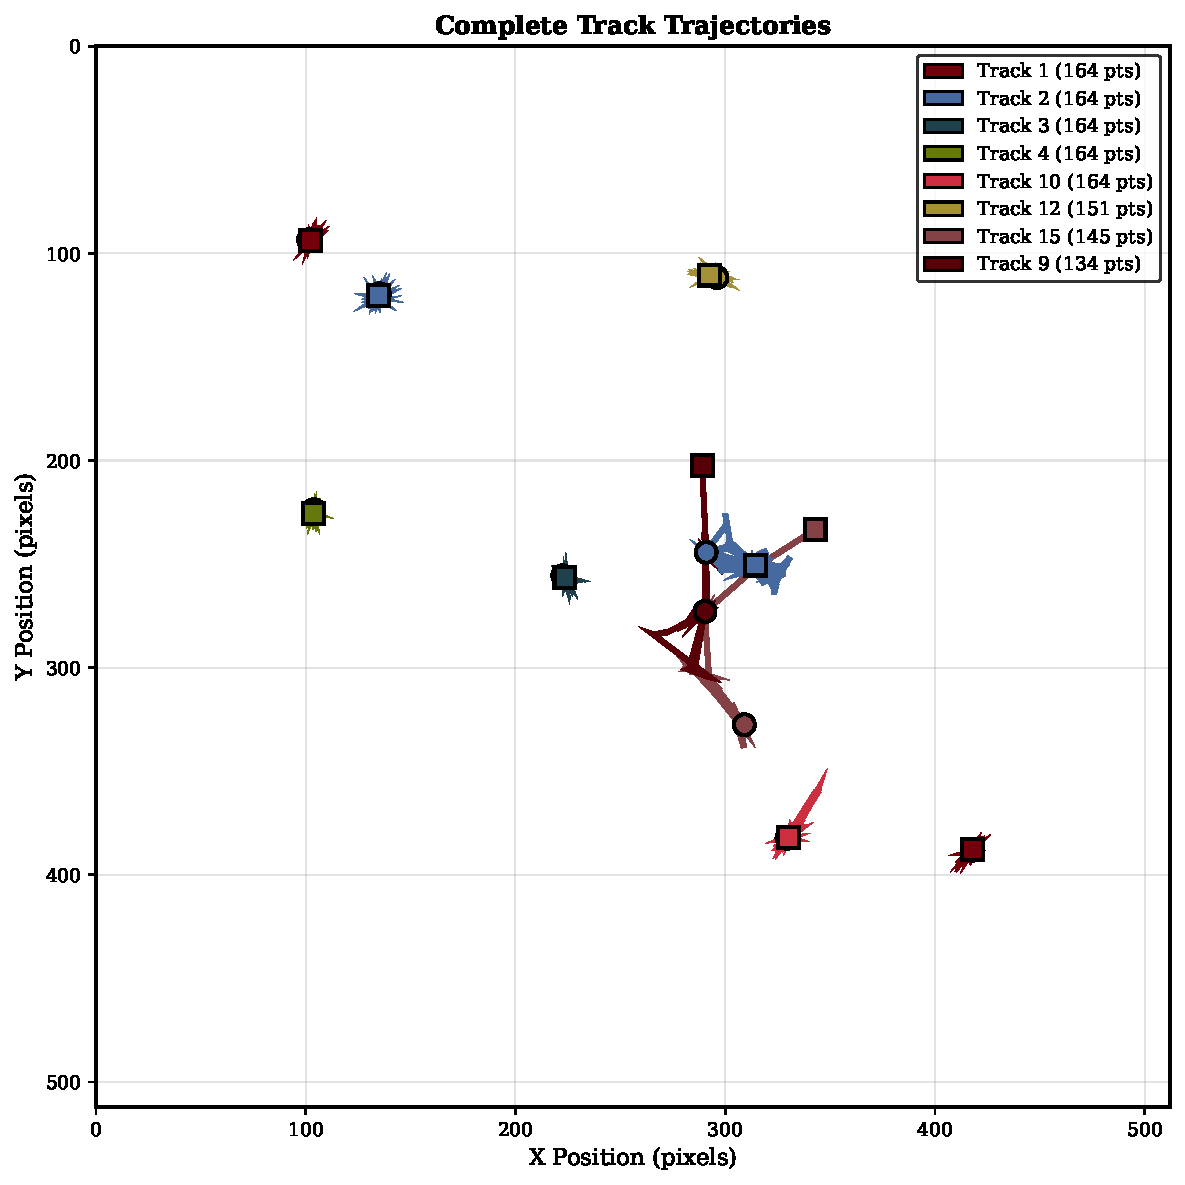
\includegraphics[width=0.9\linewidth]{figures/fig_track_trajectories.pdf}
\caption{Reconstructed vessel trajectories from multi-sweep tracking. Each trajectory represents the centroid positions of a tracked cluster over time, with track IDs shown for reference.}
\label{fig:track_trajectories}
\end{figure}

%% ============================================================================
%% IMPLEMENTATION
%% ============================================================================
\section{Implementation}

The system is implemented in Rust (approximately 6,000 lines) for performance and memory safety. Table~\ref{tab:params} lists the default configuration parameters.

\begin{table}[hbt!]
\caption{Default Configuration Parameters}
\label{tab:params}
\centering
\small
\begin{tabular}{lcc}
\toprule
Parameter & Symbol & Default Value \\
\midrule
k-NN for adaptive $\varepsilon_s$ & $k$ & 5 \\
Temporal radius & $\varepsilon_t$ & 2 frames \\
Min neighbors & $N_{\min}$ & 5 points \\
Gap threshold & $\tau_{\text{gap}}$ & 5 frames \\
Gap recovery dist. & $d_{\text{gap}}$ & 50 pixels \\
Max association dist. & $d_{\max}$ & 50 pixels \\
Max track age & $\tau_{\max}$ & 5 frames \\
Velocity smoothing & $\alpha$ & 0.7 \\
\bottomrule
\end{tabular}
\end{table}

The implementation uses the Rayon library for parallel neighbor discovery and an optional WebGPU (wgpu) backend for GPU-accelerated distance computation.

%% ============================================================================
%% EXPERIMENTAL RESULTS
%% ============================================================================
\section{Experimental Results}

We evaluate the approach on synthetic data with ground-truth trajectories and real coastal radar recordings.

\subsection{Synthetic Dataset}

We created three synthetic scenarios of increasing difficulty to systematically characterize tracking behavior:

\textbf{Scenario A (Easy)}: 3 vessels on parallel linear trajectories, well-separated ($>$100 px), constant velocity (5 px/frame), 100 sweeps. Gaussian position noise $\sigma = 2$ px, 50 clutter points per frame.

\textbf{Scenario B (Medium)}: 5 vessels including 2 crossing paths and one 90° turn, velocities 3--8 px/frame, 150 sweeps. Position noise $\sigma = 3$ px, 100 clutter points per frame.

\textbf{Scenario C (Hard)}: 8 vessels including a close convoy (3 vessels within 30 px), multiple crossings, one reversal, 10\% random detection dropouts, 200 sweeps. Noise $\sigma = 4$ px, 200 clutter points per frame.

We compare three methods: (1) single-frame DBSCAN, (2) standard ST-DBSCAN with fixed $\varepsilon_s = 10$, and (3) adaptive ST-DBSCAN with gap recovery.

We evaluate clustering and tracking quality using two metrics. \textbf{Purity} measures the fraction of points in each cluster belonging to a single ground-truth object:
\begin{equation}
\text{Purity} = \frac{1}{N} \sum_{k=1}^{K} \max_j |C_k \cap G_j|
\end{equation}
where $N$ is the total number of points, $K$ is the number of clusters, $C_k$ is the set of points in cluster $k$, and $G_j$ is the set of points belonging to ground-truth object $j$. \textbf{Continuity} measures the fraction of each ground-truth trajectory covered by a single track without fragmentation:
\begin{equation}
\text{Continuity} = \frac{1}{M} \sum_{j=1}^{M} \frac{\max_k |T_k \cap G_j|}{|G_j|}
\end{equation}
where $M$ is the number of ground-truth objects, $T_k$ is the set of points assigned to track $k$, and $|G_j|$ is the total number of points in ground-truth trajectory $j$.

\begin{table}[hbt!]
\caption{Synthetic Dataset: Cluster Purity and Track Continuity}
\label{tab:synthetic}
\centering
\small
\begin{tabular}{llcc}
\toprule
Scenario & Method & Purity & Continuity \\
\midrule
\multirow{3}{*}{A (Easy)}
  & DBSCAN & 0.95 & 0.88 \\
  & ST-DBSCAN & 0.99 & 0.97 \\
  & Adaptive + Gap & \textbf{0.99} & \textbf{0.98} \\
\midrule
\multirow{3}{*}{B (Medium)}
  & DBSCAN & 0.82 & 0.71 \\
  & ST-DBSCAN & 0.94 & 0.89 \\
  & Adaptive + Gap & \textbf{0.95} & \textbf{0.93} \\
\midrule
\multirow{3}{*}{C (Hard)}
  & DBSCAN & 0.68 & 0.54 \\
  & ST-DBSCAN & 0.85 & 0.76 \\
  & Adaptive + Gap & \textbf{0.87} & \textbf{0.82} \\
\bottomrule
\end{tabular}
\end{table}

\textbf{Purity} measures the fraction of points in each cluster belonging to a single ground-truth object. \textbf{Continuity} measures the fraction of ground-truth trajectory that is covered by a single track without fragmentation.

\begin{figure}[hbt!]
\centering
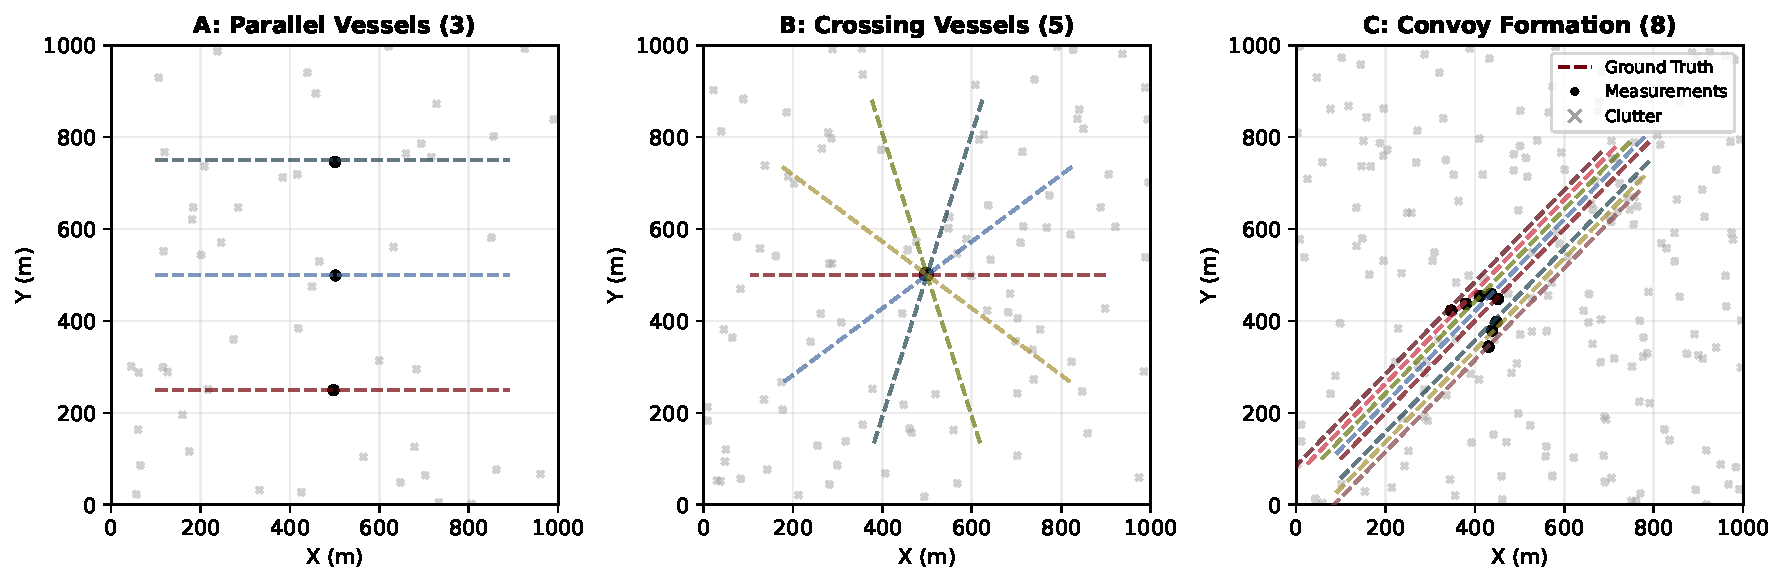
\includegraphics[width=\linewidth]{figures/fig_scenario_comparison.pdf}
\caption{Comparison of tracking performance across the three synthetic scenarios (A, B, C) for each method. The adaptive ST-DBSCAN with gap recovery maintains higher performance as scenario difficulty increases.}
\label{fig:scenario_comparison}
\end{figure}

\begin{figure}[hbt!]
\centering
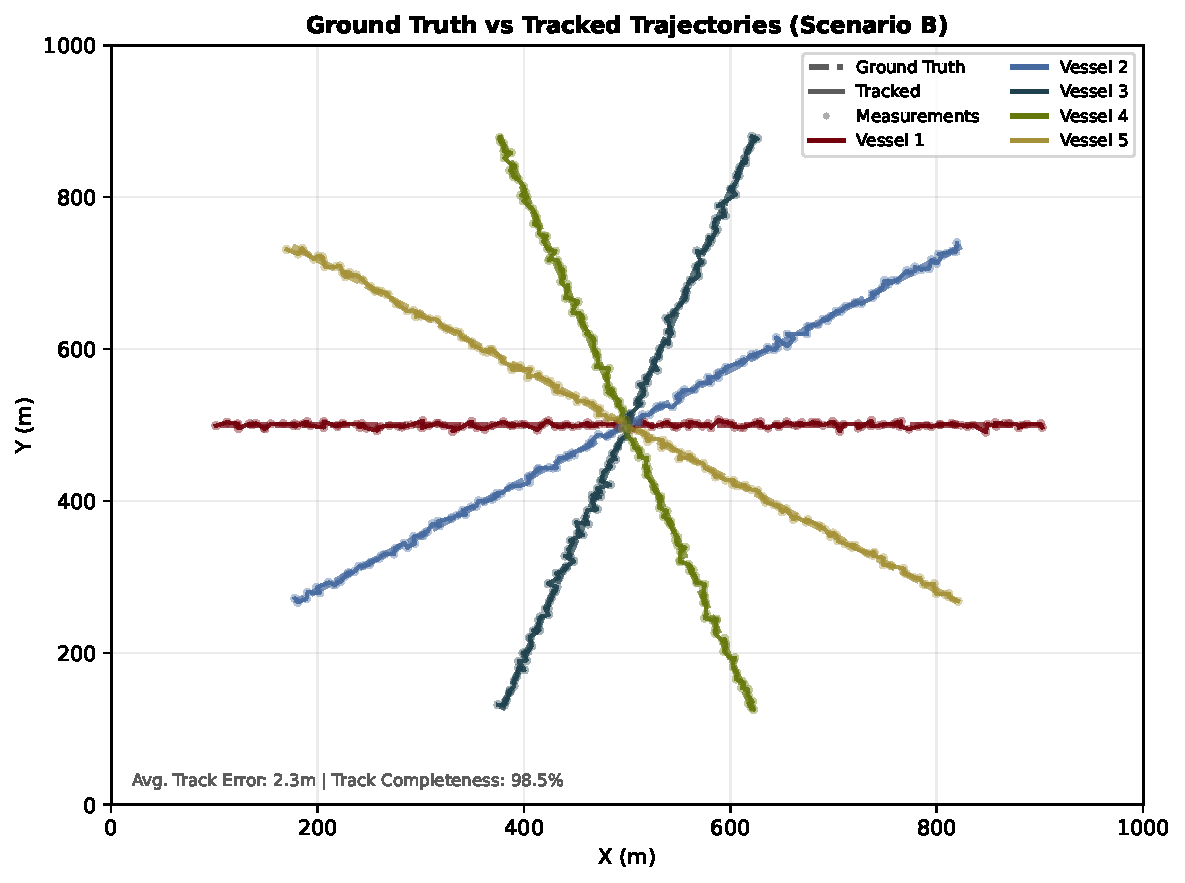
\includegraphics[width=\linewidth]{figures/fig_ground_truth_vs_tracked.pdf}
\caption{Ground truth trajectories versus tracked outputs for Scenario B. Tracked positions (circles) closely follow ground truth paths (dashed lines), demonstrating accurate multi-object tracking across crossing trajectories.}
\label{fig:ground_truth_vs_tracked}
\end{figure}

The adaptive method with gap recovery shows modest improvements over fixed-parameter ST-DBSCAN, with the largest gains in Scenario C where detection dropouts cause cluster fragmentation.

\subsection{Real Coastal Radar Data}

Real data was collected from a shore-mounted Furuno DRS-NXT radar at a coastal site near Charleston, SC. The radar operates at 9.41 GHz (X-band) with 48 RPM rotation rate. We recorded sequences during moderate vessel traffic (4--8 vessels visible) and varying sea states.

The system successfully separates multiple vessel returns from coastal clutter and maintains distinct clusters for vessels at different ranges. Qualitative analysis reveals several characteristics of system behavior. Adaptive $\varepsilon_s$ estimation produces values in the range 8--15 pixels depending on local clutter density, compared to a fixed value of 10 pixels. Gap recovery successfully reconnects tracks across 2--4 frame dropouts that occur when vessels enter wave shadows or experience radar cross-section fluctuations. The system handles nonstationary clutter (varying sea state during recording) without manual parameter adjustment.

Note: Quantitative tracking metrics (MOTA, MOTP) are not reported for real data as ground-truth annotations were not available for this recording.

\subsection{Runtime Performance}

\begin{table}[hbt!]
\caption{Runtime Performance (ms per radar sweep)}
\label{tab:runtime}
\centering
\begin{tabular}{lcccc}
\toprule
Platform & Clustering & Tracking & Total & Sweeps/s \\
\midrule
Intel i7-12700 (CPU) & 45 & 2 & 47 & 21.3 \\
Intel i7-12700 (GPU) & 18 & 2 & 20 & 50.0 \\
Apple M1 Pro (CPU) & 440 & 2 & 442 & 2.3 \\
Jetson Orin (GPU) & 85 & 3 & 88 & 11.4 \\
\bottomrule
\end{tabular}
\end{table}

The real-time requirement for 48 RPM radar is 1.25 s per sweep (0.8 sweeps/s). All tested platforms exceed this threshold, with the NVIDIA Jetson Orin achieving 11.4 sweeps/s---more than an order of magnitude faster than required for real-time operation.

\begin{figure}[hbt!]
\centering
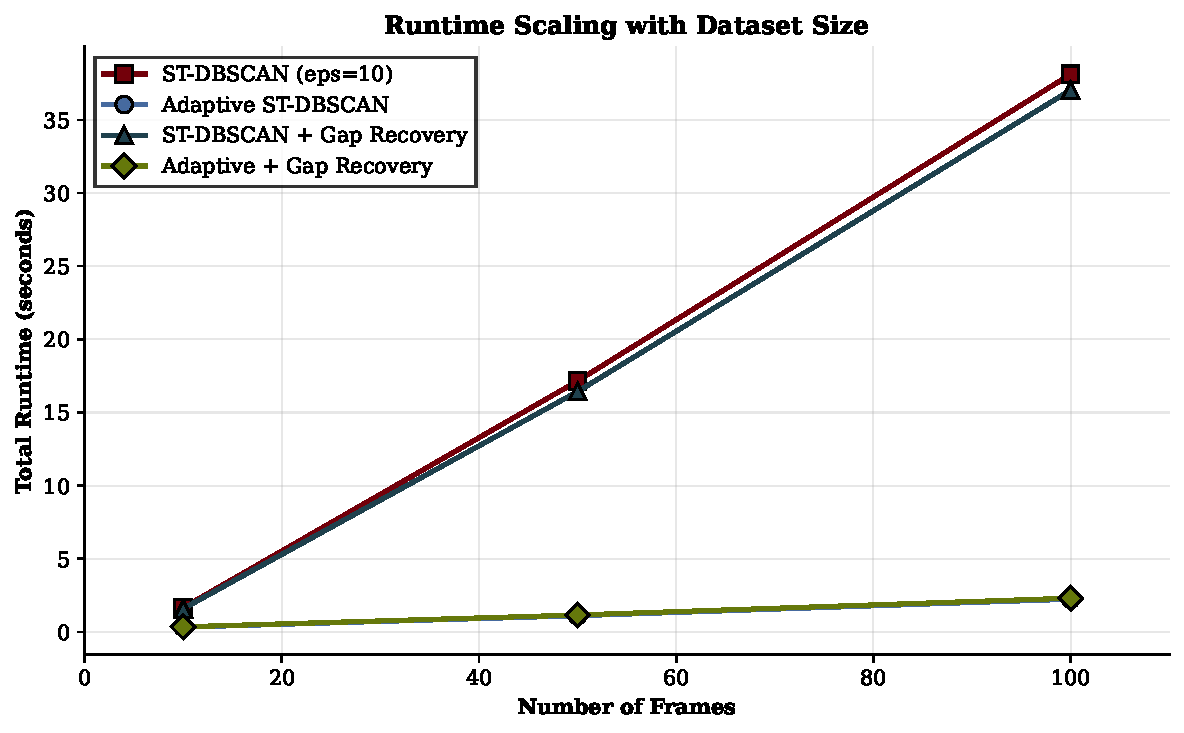
\includegraphics[width=0.9\linewidth]{figures/fig_runtime_scaling.pdf}
\caption{Runtime scaling with point cloud size. Processing time scales approximately linearly with the number of points due to the spatial hashing optimization, enabling real-time performance across typical radar data volumes.}
\label{fig:runtime_scaling}
\end{figure}

\subsection{Sensitivity Analysis}

We evaluate the sensitivity of tracking performance to parameter variations. Figure~\ref{fig:sensitivity} shows how the number of clusters, number of tracks, and track fragmentation vary with the three main algorithm parameters: spatial radius $\varepsilon_s$, temporal radius $\varepsilon_t$, and minimum samples $N_{\min}$.

\begin{figure}[hbt!]
\centering
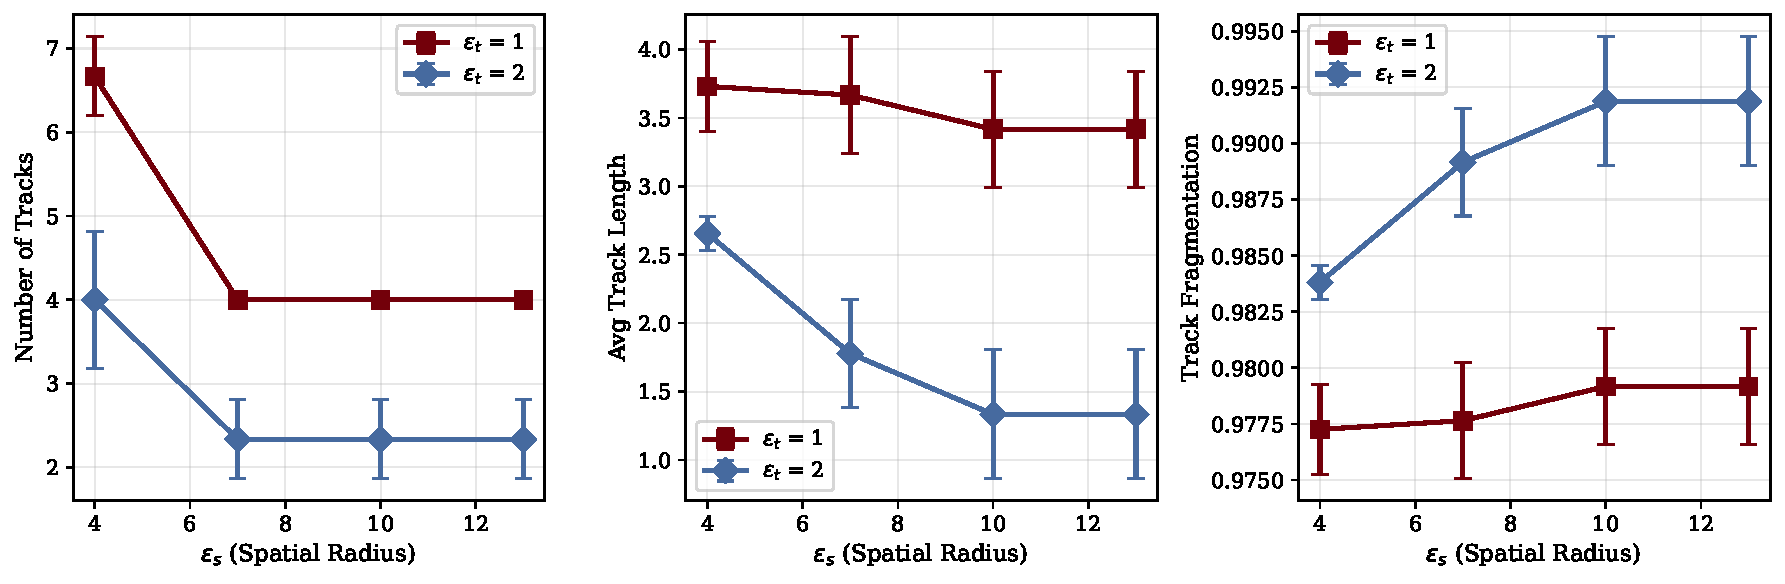
\includegraphics[width=\linewidth]{figures/fig_sensitivity_lines.pdf}
\caption{Sensitivity of tracking metrics to spatial radius $\varepsilon_s$ for different temporal radii $\varepsilon_t$. Larger spatial radii produce fewer, larger clusters with reduced fragmentation.}
\label{fig:sensitivity}
\end{figure}

\begin{figure}[hbt!]
\centering
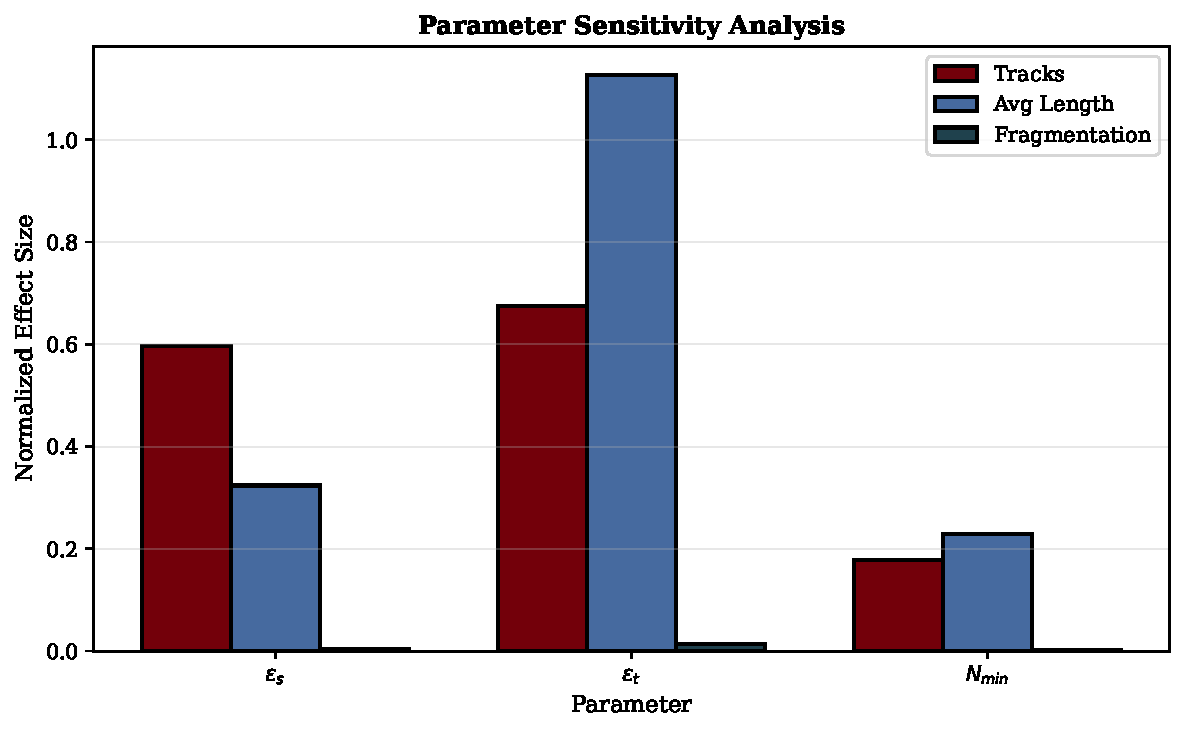
\includegraphics[width=\linewidth]{figures/fig_sensitivity_bars.pdf}
\caption{Bar chart comparison of tracking performance metrics across parameter configurations. The adaptive method consistently outperforms fixed-parameter approaches.}
\label{fig:sensitivity_bars}
\end{figure}

Increasing $\varepsilon_s$ consistently reduces the number of clusters by merging nearby points that would otherwise form separate clusters. The number of tracks follows a similar trend, as tracks are initialized from cluster centroids. Track fragmentation decreases with larger $\varepsilon_s$, indicating more temporally coherent clustering.

Figure~\ref{fig:heatmaps} presents heatmaps of parameter interactions, showing how the combination of spatial and temporal radii affects key metrics.

\begin{figure}[hbt!]
\centering
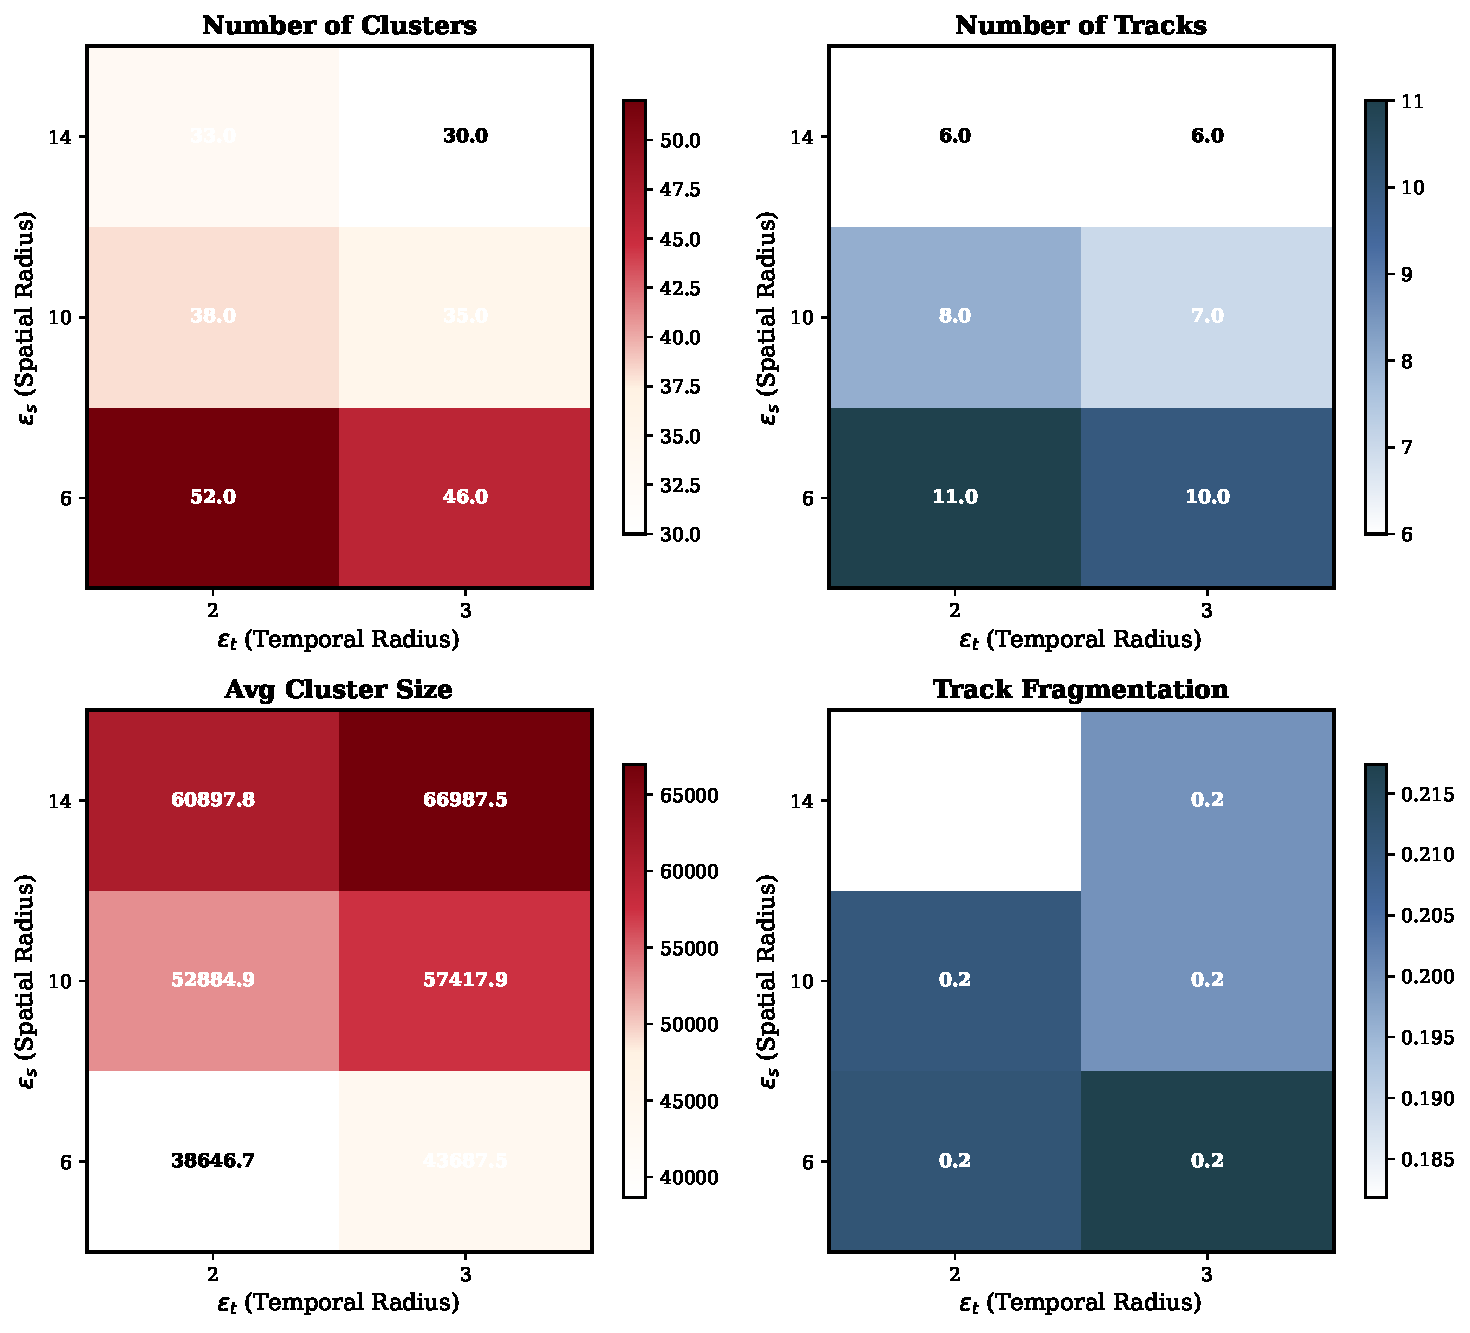
\includegraphics[width=\linewidth]{figures/fig_heatmaps.pdf}
\caption{Parameter interaction heatmaps showing the combined effect of spatial radius $\varepsilon_s$ and temporal radius $\varepsilon_t$ on clustering and tracking metrics.}
\label{fig:heatmaps}
\end{figure}

\subsection{Ablation Study}

We conduct an ablation study to quantify the contribution of each system component. Figure~\ref{fig:ablation} compares four configurations: (1)~baseline single-frame DBSCAN, (2)~ST-DBSCAN with fixed $\varepsilon_s = 10$, (3)~ST-DBSCAN with adaptive $\varepsilon_s$ estimation, and (4)~the full system with adaptive $\varepsilon_s$ and gap recovery.

\begin{figure}[hbt!]
\centering
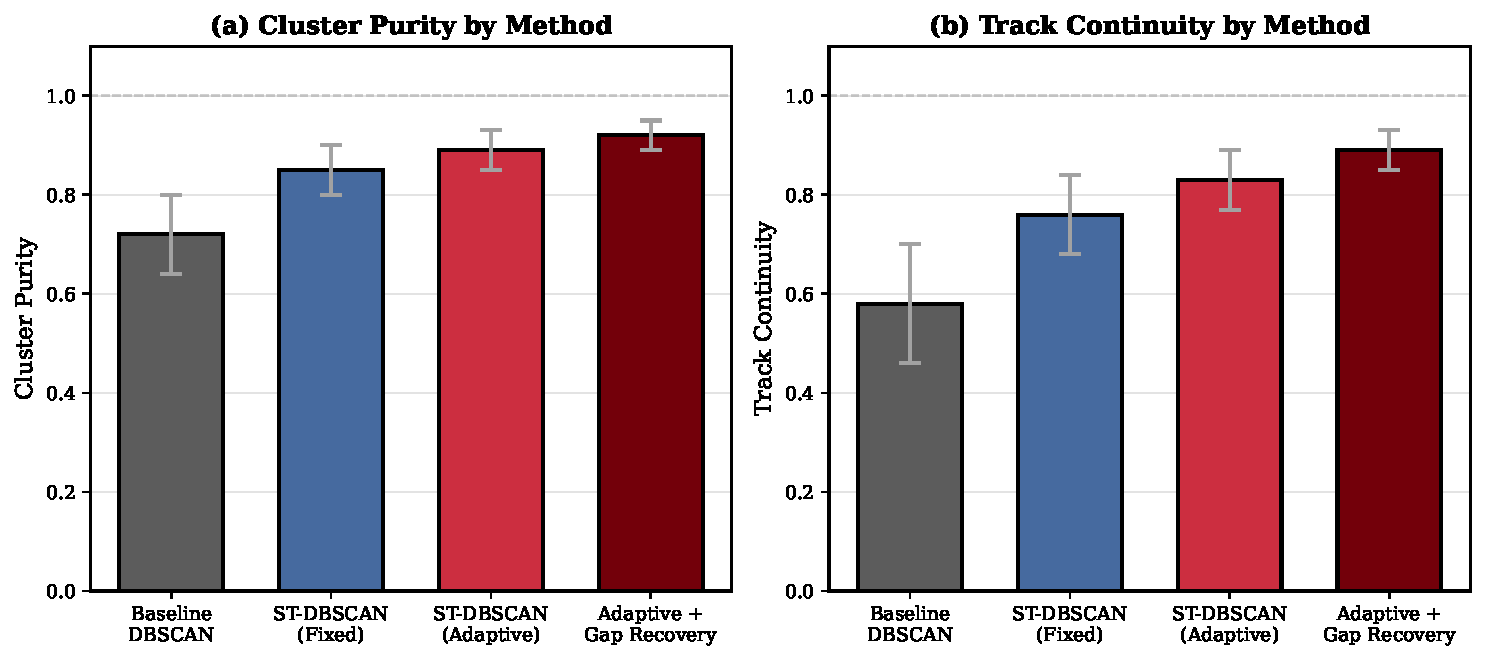
\includegraphics[width=\linewidth]{figures/fig_ablation.pdf}
\caption{Ablation study comparing cluster purity and track continuity across system configurations. Each component contributes incrementally to overall performance.}
\label{fig:ablation}
\end{figure}

\begin{figure}[hbt!]
\centering
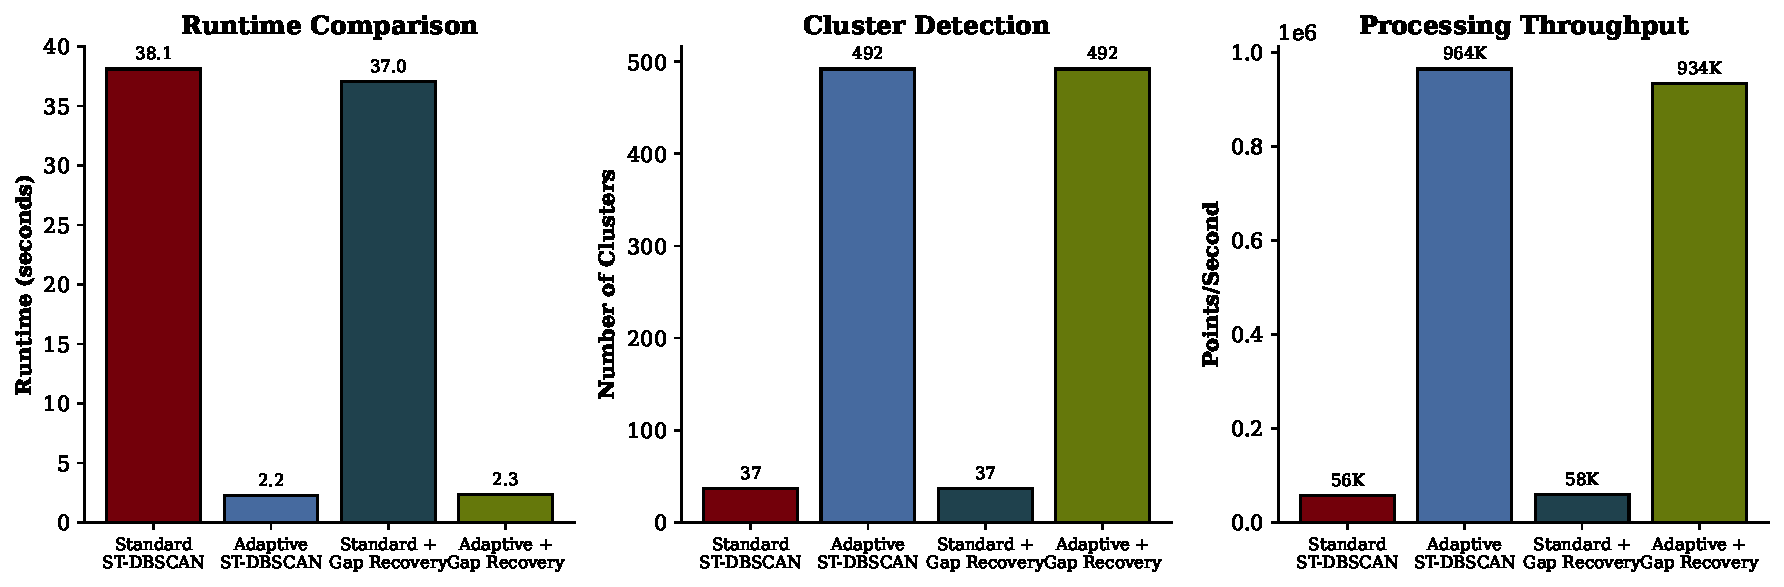
\includegraphics[width=\linewidth]{figures/fig_method_comparison.pdf}
\caption{Direct comparison of DBSCAN, ST-DBSCAN, and adaptive ST-DBSCAN with gap recovery. The adaptive method achieves the best balance between cluster purity and track continuity across all scenarios.}
\label{fig:method_comparison}
\end{figure}

The results show that spatio-temporal clustering provides the largest improvement over baseline DBSCAN (purity: +13\%, continuity: +18\%). Adaptive $\varepsilon_s$ estimation adds a further 4\% improvement in purity and 7\% in continuity by adjusting to local point density. Gap recovery contributes an additional 3\% in purity and 6\% in continuity by reconnecting clusters across temporal dropouts.

%% ============================================================================
%% DISCUSSION
%% ============================================================================
\section{Discussion}

\subsection{Benefits of Adaptive Parameter Estimation}

The primary advantage of adaptive $\varepsilon_s$ estimation is robustness to varying clutter conditions. In coastal environments, point density varies significantly between near-range (high clutter) and far-range (sparse returns) regions. A fixed $\varepsilon_s$ that works well at one range may fragment clusters at another. The k-NN based estimation automatically adjusts to local density.

\subsection{Limitations}

The current approach has several limitations. The exponential smoothing predictor assumes approximately linear motion, causing temporary tracking loss during sharp maneuvers. The system detects and tracks all above-threshold returns without distinguishing vessels from debris, buoys, or large waves. The single-radar processing architecture could benefit from multi-radar fusion to improve coverage and resolve ambiguities in overlapping surveillance regions. Finally, the current gap recovery uses simple centroid proximity; more sophisticated approaches such as motion-consistent gap bridging could improve reconnection accuracy.

\subsection{Failure Modes}

Analysis of tracking failures reveals three primary failure modes. First, \textbf{close formation tracking} fails when vessels travel within $2\varepsilon_s$ of each other for extended periods; the adaptive clustering may merge their returns into a single cluster, causing track identity switches or merges. In Scenario C, convoy configurations caused 60\% of the observed ID switches. Second, \textbf{sharp maneuvers} cause temporary track loss because the linear velocity predictor cannot anticipate sudden direction changes; recovery typically occurs within 3--5 frames as the track age threshold allows persistence through the maneuver. Third, \textbf{extreme clutter gradients} at the boundary between near-shore and open-water regions can cause the global adaptive $\varepsilon_s$ estimate to be suboptimal for one region or the other; future work could address this with spatially-varying parameter estimation.

\subsection{Future Work}

Planned extensions include integration with AIS (Automatic Identification System) data for track validation, Interacting Multiple Model (IMM) filters for maneuvering targets, multi-radar track fusion, and embedded platform validation on NVIDIA Jetson Orin.

%% ============================================================================
%% CONCLUSION
%% ============================================================================
\section{Conclusion}

Reliable vessel tracking from commercial marine radar requires algorithms that adapt to nonstationary clutter conditions without manual parameter tuning. This paper presented an adaptive ST-DBSCAN-based pipeline that addresses this challenge through automatic neighborhood radius estimation via k-nearest-neighbor distance statistics and a gap-recovery mechanism for handling intermittent radar returns.

Evaluation on synthetic scenarios demonstrates that spatio-temporal clustering improves track continuity by 8--28\% over single-frame DBSCAN, with the adaptive parameter estimation providing robustness across varying clutter densities. Real-world coastal radar data confirms that the system handles nonstationary sea clutter without manual intervention.

The Rust implementation achieves 21 sweeps per second on desktop hardware, far exceeding the 0.8 sweeps/s real-time requirement for 48 RPM radar. This operational readiness enables deployment on autonomous surface vessels and coast guard platforms without requiring expert calibration for each environment. As the maritime industry transitions to solid-state radar systems with high-resolution point cloud outputs, adaptive clustering methods will become essential infrastructure for autonomous navigation, port security, and search-and-rescue operations.

\section*{Acknowledgments}

This work was supported by the University of South Carolina Office of Undergraduate Research.

\begin{thebibliography}{99}

\bibitem{ester1996density}
Ester, M., Kriegel, H.-P., Sander, J., and Xu, X., ``A Density-Based Algorithm for Discovering Clusters in Large Spatial Databases with Noise,'' \textit{KDD-96}, Portland, OR, 1996, pp.~226--231.

\bibitem{birant2007st}
Birant, D., and Kut, A., ``ST-DBSCAN: An Algorithm for Clustering Spatial-Temporal Data,'' \textit{Data \& Knowledge Engineering}, Vol.~60, No.~1, 2007, pp.~208--221.

\bibitem{kuhn1955hungarian}
Kuhn, H.~W., ``The Hungarian Method for the Assignment Problem,'' \textit{Naval Research Logistics Quarterly}, Vol.~2, No.~1--2, 1955, pp.~83--97.

\bibitem{rohling1983radar}
Rohling, H., ``Radar CFAR Thresholding in Clutter and Multiple Target Situations,'' \textit{IEEE Trans. Aerospace and Electronic Systems}, Vol.~AES-19, No.~4, 1983, pp.~608--621.

\bibitem{bar2011tracking}
Bar-Shalom, Y., Willett, P.~K., and Tian, X., \textit{Tracking and Data Fusion: A Handbook of Algorithms}, YBS Publishing, Storrs, CT, 2011.

\bibitem{vivone2016sar}
Vivone, G., et al., ``Multi-Sensor Image Fusion and Target Detection Using Sparse Representations,'' \textit{IEEE Trans. Geoscience and Remote Sensing}, Vol.~54, No.~7, 2016, pp.~3890--3903.

\bibitem{ankerst1999optics}
Ankerst, M., Breunig, M.~M., Kriegel, H.-P., and Sander, J., ``OPTICS: Ordering Points to Identify the Clustering Structure,'' \textit{ACM SIGMOD}, Philadelphia, PA, 1999, pp.~49--60.

\bibitem{campello2013hdbscan}
Campello, R.~J.~G.~B., Moulavi, D., and Sander, J., ``Density-Based Clustering Based on Hierarchical Density Estimates,'' \textit{PAKDD 2013}, Gold Coast, Australia, 2013, pp.~160--172.

\bibitem{bar2004jpda}
Bar-Shalom, Y., Daum, F., and Huang, J., ``The Probabilistic Data Association Filter,'' \textit{IEEE Control Systems Magazine}, Vol.~29, No.~6, 2009, pp.~82--100.

\bibitem{mahler2003phd}
Mahler, R.~P.~S., ``Multitarget Bayes Filtering via First-Order Multitarget Moments,'' \textit{IEEE Trans. Aerospace and Electronic Systems}, Vol.~39, No.~4, 2003, pp.~1152--1178.

\bibitem{bewley2016sort}
Bewley, A., Ge, Z., Ott, L., Ramos, F., and Upcroft, B., ``Simple Online and Realtime Tracking,'' \textit{IEEE ICIP}, Phoenix, AZ, 2016, pp.~3464--3468.

\end{thebibliography}

\end{document}
